% Instructions to change to html version:
% Comment out:
%  minipage, multicols,columnbreak, mathbf, hrule
% Replace all: \begin{minipage}% \end{minipage} %\begin{mulicols}  %\end{mulicols}  %\columnbreak % \begin{framed} %\end{framed} %\hrule
% Search for \mathbf
% Replace $$ with \[ and $ with \(
% Enclose graphics in figure environments and add captions
% Re-tag \df environments as sections, subsections, etc.
% Command Line Code to Create html version:
%First: pdflatex -shell-escape filename.tex                                   
%Second, for each figure: inkscape "filename-figure1.pdf" -o "filename-figure1.png"
% Third: htlatex filename.tex "ht5mjlatex.cfg, charset=utf-8" " -cunihtf -utf8"
\documentclass[10pt]{article}

%\usepackage{tikz, pgf,pgfplots,wasysym,array}
%\usepackage{wasysym,array}

\usepackage{amsmath,amssymb}

\ifdefined\HCode
  \def\pgfsysdriver{pgfsys-tex4ht-updated.def}
\fi 
%\ifdefined\HCode
%  \def\pgfsysdriver{pgfsys-dvisvgm4ht.def}
%\fi 
\usepackage{tikz}
\usetikzlibrary{calc,decorations.markings,arrows}
\usepackage{pgfplots}

\pgfplotsset{compat=1.12}
\usepackage{myexternalize}
\usetikzlibrary{calc,decorations.markings,arrows}
\usepackage{framed}
\usepackage[none]{hyphenat}

\input{../../../common/1336_header_test.tex}
% \input{header.tex}

\usepackage{multirow, array}
\begin{document}



\everymath{\displaystyle}



\newcommand{\ihat}{\boldsymbol{\hat{\textbf{\i}}}}
\newcommand{\jhat}{\boldsymbol{\hat{\textbf{\j}}}}
\newcommand{\khat}{\boldsymbol{\hat{\textbf{k}}}}

\let\oldvec\vec
\renewcommand{\vec}[1]{\oldvec{\mathbf{#1}}}

\renewcommand{\u}{\vec{u}}
\renewcommand{\v}{\vec{v}}
\newcommand{\w}{\vec{w}}
\renewcommand{\r}{\vec{r}}
\renewcommand{\a}{\vec{a}}
\renewcommand{\b}{\vec{b}}

\newcommand{\grad}{\vec{\nabla}}
\newcommand{\<}{\left\langle}
\renewcommand{\>}{\right\rangle}

\renewcommand{\myTitle}{MATH 1336: Calculus III}

\renewcommand{\mySubTitle}{Section 1.1: Parametric Curves}
%~\hfill Name: \underline{~~~~~~~~~~~~~~~~~~~~~~~~~~~~~~~~~~~~~~~~~~~~~~~}

\lectTitle{\vspace*{-.5in}\myTitle}{\vspace*{.1in}\mySubTitle \vspace*{-.25in}}

%\begin{enumerate}
%
%\addtocounter{enumi}{-1}
%
%\item \textbf{Introductions \& Personalizing your Zoom Profile:}\\
%It would be great if you are able to turn your camera \& microphone when in Breakout Rooms!\\
% If you are not able to turn your camera on, please make use of the chat feature to communicate.
%\begin{enumerate}
%\item Introduce yourself and say where you are located.
%\item Go to https://seattleu.zoom.us/profile and set your name.\\ Use the first and last name you prefer. If you have enough space, consider if you want to add your pronouns or a phonetic pronunciation. It is also nice to add a picture of yourself so that people can see your face instead of just your name when your camera is not on. \\
%(If you don't already have a profile picture picked out, you may want to save that part for after class.)
%\end{enumerate}
%
%\vspace*{.2in}
%
%\hrule
%~\\
%\textbf{Work with your partners on the following problems.\\
% If you get stuck, click ``Ask for help,'' and I will join you as soon as I can.\\ 
% I will also visit rooms to check in with you to see how things are going. }\\
%
%\hrule
%\vspace*{.2in}



%\section*{13.2 - Part 1: Line Integrals wrt Arclength}

\setlength{\columnseprule}{0.4pt}
\setlength{\columnsep}{3em}

%\hspace*{-.8in}%\begin{minipage}{1.25\textwidth}
%\begin{framed}

\section*{Intro to Parametric Curves Terminology:}

%\begin{minipage}{.4\textwidth}

\begin{figure}[!h]
\includegraphics[width=\textwidth]{parametric-curve.jpeg}
\caption{Figure illustrating a general parametric curve.}
\end{figure}


%\end{minipage}
%\hspace*{.1in}
%\begin{minipage}{.6\textwidth}


 
 The \textbf{parametric equations} for the curve \(C\): 
\[
\left\lbrace\begin{matrix}
x = f(t)\\
y = g(t)
\end{matrix}
\right.
\]
give the coordinates of a point on the curve in terms the independent variable \(t\), which is referred to as the \textbf{parameter}. \\

The \textbf{parametric curve}, \(C\), can be created by tracing out points
 \((x, y) = (f(t),\ g(t))\). \\

If we are given a restricted interval for \(t\), we will only get part of the curve.
\[
x = f(t), \quad y = g(t), \quad a \leq t \leq b
\]
gives the part of the curve from the \textbf{initial point:} \((x,y) = (f(a), g(a))\) \\
to the \textbf{terminal point:} \((x,y) = (f(b), g(b))\). \\

Note that parametric curves have a direction associated with them, which is indicated by drawing an arrow in the direction of increasing \(t-\)values.

%\end{minipage}
%
%\vspace*{.1in}\hrule \vspace*{.2in}
%
%\df{\textcolor{sblack}{Line Integral of a Scalar Function with respect to Arclength:}}
%
%\[
%\int_C f(x,y)\ ds
%\]
%denotes an integral whose domain of integration is a curve \(C\) from some starting point \(A\) to an ending point \(B\).\\
%  To evaluate, we want to rewrite the integral in terms of the parameter \(t\), using the distance element \(ds = \sqrt{\left(\frac{dx}{dt}\right)^2+\left(\frac{dy}{dt}\right)^2} dt \):
%
%\[
%\int_C f(x,y)\ ds = \int_a^b f( x(t), y(t) ) \sqrt{\left(\frac{dx}{dt}\right)^2+\left(\frac{dy}{dt}\right)^2} dt 
%\]


%\end{framed}

%\end{minipage}

\section*{Example:}
\textit{Note that this example was covered in one of the pre-class videos for today's class. In the future, we will not repeat examples from the videos in class, but I will be happy to answer questions about them!}

\begin{enumerate}[{Example} 1: ]
\item Sketch the curve defined by the parametric equations, then eliminate the parameter \(t\) to obtain an equation in terms of only \(x\) and \(y\), which is referred to as a \textbf{Cartesian equation}.
\[
x = t^2 - 2t, \quad y = t+1, \quad 0 \leq t \leq 4
\]

\begin{figure}[!h]

%\begin{minipage}{.4\textwidth}
%\hspace*{-.75in}
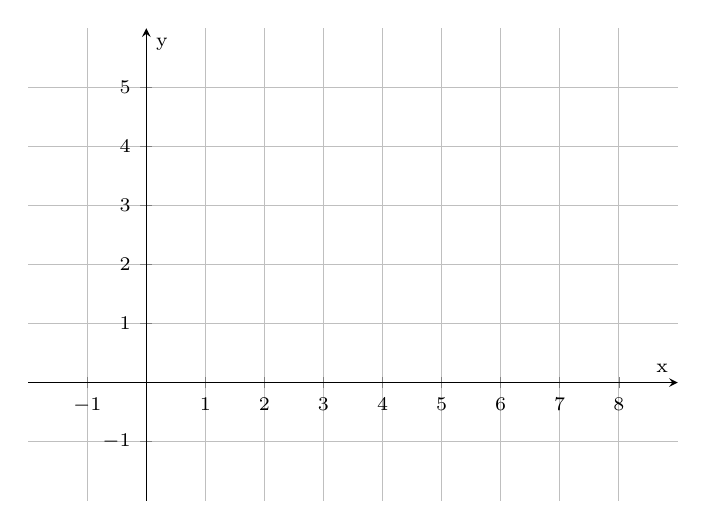
\begin{tikzpicture}
\begin{axis}[
	x=.75cm,
    y=.75cm,
	axis x line=middle,
	axis y line = middle,
	xmin=-2,xmax=9,
	ymin=-2,ymax=6,
    grid=both,
%    ticks=none,
%    yticklabels={},
%    xticklabels={},
    xtick={-1,0,...,8},
    ytick={-1,0,...,5},
    xlabel=x,
    ylabel=y,
    label style={font=\scriptsize},
    tick label style={font=\scriptsize}
]



\end{axis}
%\filldraw[fill=green!20,draw=green!50!black] (1.5cm,0cm) -- (3.75cm,0cm) arc
%(0:45:3.75cm) -- (1.065cm,1.065cm) arc (45:0:1.5cm) -- cycle;
%
%

\end{tikzpicture}
%\end{minipage}

\caption{Blank set of coordinate axes for sketching the parametric curve from Example 1.}
\end{figure}

\vfill
\noindent \textit{Followup Discussion: What do you think are some advantages of parametric equations? disadvantages?}


\end{enumerate}

\pagebreak

\section*{Group Work:}


\subsection*{Introductions:}

Introduce yourself to your neighbors. Share one unusual thing that you did over the break.


\subsection*{Work with your partners on the following problems:}
\begin{enumerate}[{Problem} 1:]


\item Sketch the curve by using the parametric equations to plot points. Indicate with an arrow the direction in which the curve is traced as \(t\) increases.
\begin{enumerate}
\item \(x = t, \qquad y = t^2, \qquad -2\leq t \leq 4\)
\item \(x = t-1, \qquad y =t^3+1, \qquad -2\leq t \leq 2\)
\item \(x = \sin(t), \qquad y = \cos^2(t), \qquad -\frac{\pi}{2} \leq t \leq\frac{\pi}{2}\)
\end{enumerate}
\vfill

\item Describe the motion of a particle with position \((x,y)\) as \(t\) varies in the given interval.
\begin{enumerate}
\item \(x = \cos(t), \qquad y = \sin(t), \qquad 0\leq t \leq 2\pi\)
\item \(x = \cos(2t), \qquad y = \sin(2t), \qquad 0\leq t \leq 2\pi\)
\item \(x = \sin \left(\tfrac{1}{2}t\right), \qquad y = \cos \left(\tfrac{1}{2}t\right), \qquad -\pi\leq t \leq \pi\)
\end{enumerate}

\vfill

\item Eliminate the parameter to find a Cartesian equation of the curve.
\begin{enumerate}
\item \(x = t, \qquad y = t^2, \qquad -2\leq t \leq 4\)
\item \(x = t-1, \qquad y =t^3+1, \qquad -2\leq t \leq 2\)
\item \(x = \sin(t), \qquad y = \cos^2(t), \qquad -\frac{\pi}{2} \leq t \leq \frac{\pi}{2}\)
\end{enumerate}
\vfill



\end{enumerate}

\end{document}
